\documentclass[12pt, titlepage, a4paper]{article}
\usepackage[utf8]{inputenc}
\usepackage{changepage}
\usepackage{prftree}
\usepackage{amssymb}
\usepackage{amsmath}
\usepackage{enumitem} 
\usepackage{graphicx}
\usepackage{wrapfig}
\usepackage[spanish]{babel}
\usepackage{dirtytalk}
\usepackage{float}

\usepackage[utf8]{inputenc}
\usepackage{changepage}
\usepackage{prftree}
\usepackage{amssymb}
\usepackage{amsmath}
\usepackage{enumitem} 
\usepackage{graphicx}
\usepackage{setspace}

\usepackage[a4paper, total={6.7in, 8in}]{geometry}

\usepackage[spanish]{babel}
\usepackage{amsthm}
\usepackage{bussproofs}
\usepackage{bm}

\usepackage{fancyhdr} % Para personalizar encabezados y pies de página

\usepackage{caption}
\usepackage{subcaption}


\title{Introducción a la Inteligencia Artificial \\
Trabajo Práctico 1: Representación y Búsqueda en Espacio de Estados }
\author{Agustín Fernández Bergé y Ramiro Gatto}
\date{14/04/2025}

%%%

\fancypagestyle{firstpage}{
    \fancyhf{}
    \setlength{\headsep}{80pt} % Ajustar la separación entre el encabezado y el contenido
    \addtolength{\topmargin}{0pt} % Ajustar el margen superior

    % \addtolength{\textheight}{1in} % Ajustar la altura del texto
    % \addtolength{\footskip}{-1.5in} % Ajustar la separación entre el pie de página y el contenido

    \fancyhead[L]{    
        \vspace{-0.8cm}
        
\includegraphics[width=0.12\textwidth]{logo.jpg}
    }
    \fancyhead[R]{\setstretch{0.8}\begin{tabular}{l}
        \textsc{\footnotesize Facultad de Ciencias Exactas, Ingeniería y Agrimensura} \\
        \textsc{\footnotesize Escuela de Ciencias Exactas y Naturales} \\
        \textsc{\footnotesize Departamento de Ciencia de la Computación} \\
        \textsc{\footnotesize Introducción a la Inteligencia Artificial} \\
    \end{tabular}}

    \fancyhead[C]{\vspace{-1.7cm}Integrantes: Agustín Fernández Bergé y Ramiro Gatto\\}

    \fancyfoot[L]{\footnotesize Trabajo Práctico 1: Representación y Búsqueda en Espacio de Estado} % Pie de página izquierdo
    \fancyfoot[R]{\footnotesize Página \thepage}
    \renewcommand{\headrulewidth}{0.4pt}
    \renewcommand{\footrulewidth}{0.4pt}
}

\pagestyle{fancy} % Activar el estilo fancyhdr
\fancyhf{} % Limpiar encabezados y pies
\setlength{\headheight}{14.49998pt} % Ajustar la altura del encabezado
\addtolength{\topmargin}{-1.5cm} % Compensar el margen superior
\addtolength{\textheight}{4.5cm} % Aumentar la altura del texto
\fancyhead[L]{Introducción a la Inteligencia Artificial} % Encabezado izquierdo
\fancyfoot[L]{\footnotesize Trabajo Práctico 1: Representación y Búsqueda en Espacio de Estado} % Pie de página izquierdo
\fancyfoot[R]{\footnotesize Página \thepage}

\renewcommand{\headrulewidth}{0.4pt} % Desactivar línea superior
\renewcommand{\footrulewidth}{0.4pt} % Desactivar línea inferior (ya usamos manualmente la línea)


%%%

\begin{document}
\maketitle

\section{Ejercicio 1}
Para implementar el algoritmo de DFS (Depth-First Search) utilizamos 
el algoritmo de búsqueda general, el cual es el siguiente:\\ 

\noindent Búsqueda General\\
\indent responde con \textbf{Solución} o \textbf{Falla}\\
\indent Lista-Nodo $\leftarrow$ Estado Inicial\\

\noindent bucle hacer\\
\indent si Lista-Nodo está vacía contestar \textbf{Falla}\\
\indent tomo NODO de Lista-Nodo\\
\indent si NODO es \textbf{meta} contestar con NODO\\
\indent Lista-Nodo $\leftarrow$ expansión NODO\\
\noindent FIN\\

En este caso, se colocan los NODOS generados al expandir, al comienzo de Lista-Nodos. 

Para lograr el comportamiento de \say{agregar NODOS al comienzo de Lista-Nodo} lo que  
decidimos utilizar fue una pila, la cual captura esa idea de agregar al inicio y sacar del inicio. 
Es decir, Lista-Nodos es una pila.\\

De esta forma, combinado el pseudo código y la pila es como implementamos 
el algoritmo de DFS. Luego al usar esta solución con el \textit{bigMaze} 
y con \textit{PositionSearchProblem} se obtiene:
\begin{verbatim}
    [SearchAgent] using function dfs
    [SearchAgent] using problem type PositionSearchProblem
    Path found with total cost of 210 in 0.02 seconds
    Search nodes expanded: 390
    Pacman emerges victorious! Score: 300
    Average Score: 300.0
    Scores:        300.0
    Win Rate:      1/1 (1.00)
    Record:        Win
\end{verbatim}

%Lo cual para nosotros en optimo

\section{Ejercicio 2}
Para la implementación de BFS (Breadth-First Search) también utilizamos el 
algoritmo de búsqueda general, solo que en este se colocan los NODOS generados 
al expandir al final de Lista-Nodos.\\

Para este comportamiento se utilizo una cola (normal), la cual permite 
agregar al final y sacar del inicio. Es decir, Lista-Nodos es una pila.
En este caso, nuevamente lo probamos con el \textit{bigMaze} y con \textit{PositionSearchProblem}
 obteniéndose:
\begin{verbatim}
    [SearchAgent] using function bfs
    [SearchAgent] using problem type PositionSearchProblem
    Path found with total cost of 210 in 0.02 seconds
    Search nodes expanded: 620
    Pacman emerges victorious! Score: 300
    Average Score: 300.0
    Scores:        300.0
    Win Rate:      1/1 (1.00)
    Record:        Win
\end{verbatim}


%Usando esta solucion se tiene lo siguiente ...
%Poner un analisis

\section{Ejercicio 3}
Para implementar UCS (Uniform Cost Search) nuevamente se utilizo el 
algoritmo de búsqueda general, solo que ahora al colocar los NODOS generados 
al expandir lo hacemos en base al costo del mismo. Agregando al inicio 
los de menor costo.\\

Para lograr esto se utilizan las colas de prioridad, siendo la prioridad 
el costo del nodo. Nuevamente probamos con el \textit{bigMaze} y con \textit{PositionSearchProblem}, 
teniéndose: 
\begin{verbatim}
    [SearchAgent] using function ucs
    [SearchAgent] using problem type PositionSearchProblem
    Path found with total cost of 210 in 0.02 seconds
    Search nodes expanded: 620
    Pacman emerges victorious! Score: 300
    Average Score: 300.0
    Scores:        300.0
    Win Rate:      1/1 (1.00)
    Record:        Win
\end{verbatim}

\section{Ejercicio 4}
\subsection{Búsqueda A*}
Recordemos que el A* utiliza una función $f(Nodo)$ de 
evaluación de la forma: $f(n) = g(n) + h(n)$ donde,
\begin{itemize}
    \item {g(n) = costo hasta llegar a n}
    \item {h(n) = costo estimado hasta la meta desde n}
    \item {f(n) = costo total de ruta pasando por n hasta la meta}
\end{itemize}

En este nuevamente utilizamos el algoritmo 
de búsqueda general 
en donde Lista-Nodos se ordena de
acuerdo al valor de $f(Nodo)$.\\

Para este caso utilizamos nuevamente las colas de prioridad, y ademas también nos 
fijamos si la heurística que se utiliza es consistente, antes de hacer la búsqueda.\\

Ahora, probamos con el \textit{bigMaze}, con \textit{PositionSearchProblem} y
 utilizando como heurística la \say{distancia de manhattan}.
teniéndose: 
\begin{verbatim}
    [SearchAgent] using function astar and heuristic manhattanHeuristic
    [SearchAgent] using problem type PositionSearchProblem
    Path found with total cost of 210 in 0.02 seconds
    Search nodes expanded: 549
    Pacman emerges victorious! Score: 300
    Average Score: 300.0
    Scores:        300.0
    Win Rate:      1/1 (1.00)
    Record:        Win
\end{verbatim}

En donde se puede observar que se corrobora la dicho en el enunciado, esto 
es que hay una diferencia de uno ~100 nodos expandidos con respecto a UCS.

\subsection{Laberinto openMaze}
En esta sección vamos a analizar las 4 forma de búsqueda que hicimos con 
el laberinto \textbf{openMaze}. El recorrido que hacen es el siguiente:

\begin{figure}[H]
    \centering
    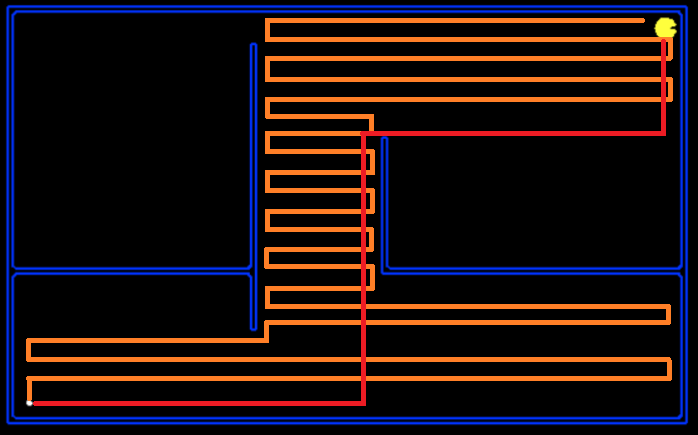
\includegraphics[width=.6\textwidth]{Imagenes/caminos.png}
    \caption{En naranja el camino del DFS, En rojo el camino del resto}
\end{figure}

Donde se tiene que todos menos el DFS siguen la misma ruta, pero 
exploran una cantidad de nodos distinto (535 en A*, 682 en UCS y en BFS, 576 en DFS). \\

A pesar de que A*, UCS y BFS expanden una cantidad distinta de nodos 
todos tienen el mismo puntaje (tardan lo mismo). Mas aun, a pesar de que DFS es uno de los que 
menos nodos expande este es el de peor puntaje (mas lento).


%%A*
%%Path found with total cost of 54 in 0.03 seconds
%%Search nodes expanded: 535
%%Pacman emerges victorious! Score: 456
%%
%%UCS
%%Path found with total cost of 54 in 0.02 seconds
%%Search nodes expanded: 682
%%Pacman emerges victorious! Score: 456
%%
%%DFS
%%Path found with total cost of 298 in 0.02 seconds
%%Search nodes expanded: 576
%%Pacman emerges victorious! Score: 212
%%
%%BFS
%%Path found with total cost of 54 in 0.02 seconds
%%Search nodes expanded: 682
%%Pacman emerges victorious! Score: 456

\section{Ejercicio 5}
\subsection{cornersProblems}
En este ejercicio tenemos que elegir una forma de representar el estado de 
tal forma que detecte si las 4 esquinas del laberinto fueron alanzadas. La 
forma que elegimos fue tomar al estado como: \textbf{(Posición actual, (Bool, Bool, Bool, Bool))}.\\

\noindent Es decir, el estado es una tupla cuyas componentes son:
\begin{itemize}
    \item {La posición actual.}
    \item {Una cuádrupla de Bool, cada uno representa una esquina del tablero en este orden: (1, 1), (1, top), (right, 1), (right, top). Al 
        principio estan todas en False.}
\end{itemize}

De esta forma cuando se llega a una esquina se cambia el False correspondiente por 
un True. Para ver si se alcanzaron todas las esquinas se hace un And generalizado 
entre todas las componentes de la cuádrupla.\\

\subsection{Posibles heurísticas}
Para el tema de las heurística se pensaron unas cuantas, y para ver si es admisible hay que 
tener en cuenta que la heurística no debe sobrestimar. La primera que se pensó fue una estilo greedy.

\ 

\noindent Punto-actual $\leftarrow$ Posicion-inicial\\
\noindent  Distancia $\leftarrow$ 0\\

\noindent bucle hacer\\
\indent si Lista-Esquinas está vacía contestar \textbf{Distancia}\\
\indent tomo ESQUINA de Lista-Esquinas-No-Visitadas\\
\indent Distancia $\leftarrow$ Distancia + distanciaManhattan(Punto-actual, ESQUINA)\\
\noindent FIN\\

Es decir, se calcula la distancia de manhattan entre el punto actual y la esquina
mas cercana, y se suma a la distancia total. Luego se repite el proceso hasta que no haya mas esquinas.
Esta heurística es valida pero puede elegir rutas no optimas en ciertas situaciones(por ejemplo, en un escenario
donde no hay paredes), por lo que no es admisible.\\

La siguiente forma fue considerar la cantidad de esquinas no visitadas. Esta heurística es consistente, ya que
la cantidad de esquinas no visitadas en cada paso disminuye en como mucho una unidad, por lo tanto es admisible.
Sin embargo la estimación del costo a la solución es demasiado optimista, por lo que la cantidad de nodos expandidos
disminuye muy poco.\\

También se intento repetir la primera heurística pero usando la distancia euclidea y la distancia con la norma
infinito. En algunos laberintos no se cumplió la propiedad de consistencia usando la distancia euclidea pero si
se mantuvo usando la distancia con norma infinito. Sin embargo es posible que haya algunos layouts donde existan
un par de estados donde la propiedad de consistencia se rompa, por lo que descartamos esta heurística.\\

La ultima heurística que pensamos fue, a partir de la posición actual, revisar todas las formas posibles
de visitar las esquinas, calcular la distancia recorrida total de cada recorrido (usando distancia de manhattan) y devolver la menor de todas
ellas.

Para una posición inicial S solamente hay que visitar 4 esquinas, por lo que solo hay que revisar 4! = 24 posibles
ordenes. Además, se pueden memorizar algunos resultados para mejorar la velocidad de computo de la heurística (aunque
esto también gasta más memoria). Esta heurística es la resolución de una restricción del problema a cuando no hay
paredes en el laberinto, asi que es esperable que sea consistente y de hecho lo es. La heurística es consistente ya que en cada paso la 
distancia a la solución varia en a lo sumo 1 paso, dado que el costo de ir de un nodo a otro es de 1, la heurística cumple la propiedad de
consistencia. Además disminuye mucho la cantidad de nodos explorados (741 nodos para la solución optima vs 1966 nodos
usando búsqueda de costo uniforme).

\section{Ejercicio 6}
La heurística no trivial consistente elegida para resolver el problema de comer todas las pastillas en las esquinas
es equivalente a aquella que revisa todos los ordenes para visitar las esquinas y elige el menor, solo que es mas eficiente
ya que evita revisar algunos recorridos no óptimos.\\

Resulta que la primera heurística que siempre intenta visitar la esquina mas cercana obtiene la respuesta optima
a visitar las esquinas de un tablero sin paredes cuando la casilla de partida es una de las esquinas. Vimos que esto es asi
analizando el escenario de un laberinto sin paredes donde hay que visitar 3, 2 o 1 esquina.\\

Si $S$ es la posición inicial y $A,B,C \text{ y } D$ son las esquinas entonces los recorridos posibles entran en alguno de estos 4 esquemas:

\begin{itemize}
    \item $S\rightarrow A \rightarrow \dots$
    \item $S\rightarrow B \rightarrow \dots$
    \item $S\rightarrow C \rightarrow \dots$
    \item $S\rightarrow D \rightarrow \dots$
\end{itemize}

Los subrecorridos que siguen desde las esquinas $A,B,C \text{ y } D$ pueden resolverse optimamente usando la primera heurística, por lo que
solo hay que revisar cuatro recorridos posibles.\\

Asi que la heurística final consiste en el siguiente algoritmo:\\

\noindent  Distancia $\leftarrow$ $\infty$\\

\noindent PARA Esquina EN Lista-Esquinas-No-Visitadas\\
\indent Lista' $\leftarrow$ Lista-Esquinas\\
\indent ELIMINAR Esquina de Lista'\\
\indent Distancia $\leftarrow$ MINIMO(Distancia, distanciaManhattan(Posicion-Actual, Esquina) + busquedaGreedy(Lista'))\\
\noindent FIN\\

Donde busquedaGreedy es la heurística que siempre busca visitar la esquina mas cercana, calculando distancias usando
la distancia de manhattan.


\section{Ejercicio 7}

La heurística elegida para ejercicio 7 consiste en dividir el tablero en cuadriculas no superponibles (en el 
código son 16 cuadriculas, pero puede ser cualquier potencia de 2). En esta division posiblemente halla 
cuadriculas que no tengan pastillas ya otras que si. A la hora de calcular la heurística, se calcula el largo 
del mínimo camino que visita todas las cuadriculas que tienen pastillas (ignorando las paredes del laberinto).\\

Esta heurística surgió de la idea de generalizar el problema de visitar las 4 esquinas del tablero al problema
de comer todas las pastillas. En este caso cada cuadricula representa una \say{esquina} a visitar, solo que las 
cuadriculas ocupan mas espacio.\\

Para mejorar la heurística, se restringe el tamaño de las cuadriculas para que haya al menos dos esquinas 
opuestas que tengan pastillas. Además algunos resultados pueden calcularse más de una vez por lo que se 
memorizan los resultados y calculados para mejorar la velocidad de computo(a costa de usar mas memoria). 
La heurística se acerca mas a la solución real a medida que se aumentan las cuadriculas, pero también aumenta
el tiempo de computo y la memoria utilizada.\\

\begin{figure}[H]
    \begin{subfigure}{0.5\textwidth}
    \centering
    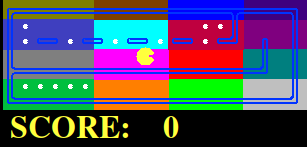
\includegraphics[width=.9\textwidth]{Imagenes/Captura desde 2025-04-09 20-07-23.png}
    \caption{Por ejemplo, para el layout trickySearch, el laberinto se divide en 16 cuadriculas.}
    \end{subfigure}%
    \begin{subfigure}[t]{0.5\textwidth}
    \centering
    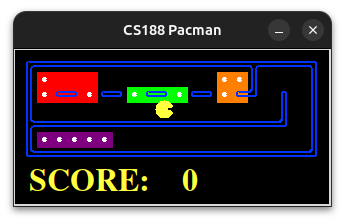
\includegraphics[width=.9\textwidth]{Imagenes/image.png}
    \caption{Si se eliminan las cuadriculas sin pastillas y se restringe el tamaño de las cuadriculas restantes, entonces solo quedan 4 cuadriculas.}
    \end{subfigure}
\end{figure}



%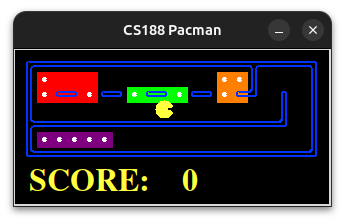
\includegraphics[width=.8\textwidth]{Imagenes/image.png}\\

El mínimo camino que visita todas las cuadriculas consta de 17 pasos, mientras
que el costo real de comer todas las pastillas es de 60 pasos. Usando esta
heurística el agente encuentra la solución en aproximadamente 0.8 segundos
explorando 9086 nodos.\\

La heurística es admisible porque un recorrido que tiene que comer todas las
pastillas como mínimo tiene que visitar todas las cuadriculas (y siempre donde
hay una cuadricula hay por lo menos 1 pastilla). Además es consistente porque en cada paso la distancia a la solución varia en solo 1 paso.\\

\end{document}